% Options for packages loaded elsewhere
\PassOptionsToPackage{unicode}{hyperref}
\PassOptionsToPackage{hyphens}{url}
%
\documentclass[
]{article}
\usepackage{lmodern}
\usepackage{amssymb,amsmath}
\usepackage{ifxetex,ifluatex}
\ifnum 0\ifxetex 1\fi\ifluatex 1\fi=0 % if pdftex
  \usepackage[T1]{fontenc}
  \usepackage[utf8]{inputenc}
  \usepackage{textcomp} % provide euro and other symbols
\else % if luatex or xetex
  \usepackage{unicode-math}
  \defaultfontfeatures{Scale=MatchLowercase}
  \defaultfontfeatures[\rmfamily]{Ligatures=TeX,Scale=1}
\fi
% Use upquote if available, for straight quotes in verbatim environments
\IfFileExists{upquote.sty}{\usepackage{upquote}}{}
\IfFileExists{microtype.sty}{% use microtype if available
  \usepackage[]{microtype}
  \UseMicrotypeSet[protrusion]{basicmath} % disable protrusion for tt fonts
}{}
\makeatletter
\@ifundefined{KOMAClassName}{% if non-KOMA class
  \IfFileExists{parskip.sty}{%
    \usepackage{parskip}
  }{% else
    \setlength{\parindent}{0pt}
    \setlength{\parskip}{6pt plus 2pt minus 1pt}}
}{% if KOMA class
  \KOMAoptions{parskip=half}}
\makeatother
\usepackage{xcolor}
\IfFileExists{xurl.sty}{\usepackage{xurl}}{} % add URL line breaks if available
\IfFileExists{bookmark.sty}{\usepackage{bookmark}}{\usepackage{hyperref}}
\hypersetup{
  pdftitle={Ökonometria},
  pdfauthor={Granát Marcell},
  hidelinks,
  pdfcreator={LaTeX via pandoc}}
\urlstyle{same} % disable monospaced font for URLs
\usepackage[margin=1in]{geometry}
\usepackage{color}
\usepackage{fancyvrb}
\newcommand{\VerbBar}{|}
\newcommand{\VERB}{\Verb[commandchars=\\\{\}]}
\DefineVerbatimEnvironment{Highlighting}{Verbatim}{commandchars=\\\{\}}
% Add ',fontsize=\small' for more characters per line
\usepackage{framed}
\definecolor{shadecolor}{RGB}{248,248,248}
\newenvironment{Shaded}{\begin{snugshade}}{\end{snugshade}}
\newcommand{\AlertTok}[1]{\textcolor[rgb]{0.94,0.16,0.16}{#1}}
\newcommand{\AnnotationTok}[1]{\textcolor[rgb]{0.56,0.35,0.01}{\textbf{\textit{#1}}}}
\newcommand{\AttributeTok}[1]{\textcolor[rgb]{0.77,0.63,0.00}{#1}}
\newcommand{\BaseNTok}[1]{\textcolor[rgb]{0.00,0.00,0.81}{#1}}
\newcommand{\BuiltInTok}[1]{#1}
\newcommand{\CharTok}[1]{\textcolor[rgb]{0.31,0.60,0.02}{#1}}
\newcommand{\CommentTok}[1]{\textcolor[rgb]{0.56,0.35,0.01}{\textit{#1}}}
\newcommand{\CommentVarTok}[1]{\textcolor[rgb]{0.56,0.35,0.01}{\textbf{\textit{#1}}}}
\newcommand{\ConstantTok}[1]{\textcolor[rgb]{0.00,0.00,0.00}{#1}}
\newcommand{\ControlFlowTok}[1]{\textcolor[rgb]{0.13,0.29,0.53}{\textbf{#1}}}
\newcommand{\DataTypeTok}[1]{\textcolor[rgb]{0.13,0.29,0.53}{#1}}
\newcommand{\DecValTok}[1]{\textcolor[rgb]{0.00,0.00,0.81}{#1}}
\newcommand{\DocumentationTok}[1]{\textcolor[rgb]{0.56,0.35,0.01}{\textbf{\textit{#1}}}}
\newcommand{\ErrorTok}[1]{\textcolor[rgb]{0.64,0.00,0.00}{\textbf{#1}}}
\newcommand{\ExtensionTok}[1]{#1}
\newcommand{\FloatTok}[1]{\textcolor[rgb]{0.00,0.00,0.81}{#1}}
\newcommand{\FunctionTok}[1]{\textcolor[rgb]{0.00,0.00,0.00}{#1}}
\newcommand{\ImportTok}[1]{#1}
\newcommand{\InformationTok}[1]{\textcolor[rgb]{0.56,0.35,0.01}{\textbf{\textit{#1}}}}
\newcommand{\KeywordTok}[1]{\textcolor[rgb]{0.13,0.29,0.53}{\textbf{#1}}}
\newcommand{\NormalTok}[1]{#1}
\newcommand{\OperatorTok}[1]{\textcolor[rgb]{0.81,0.36,0.00}{\textbf{#1}}}
\newcommand{\OtherTok}[1]{\textcolor[rgb]{0.56,0.35,0.01}{#1}}
\newcommand{\PreprocessorTok}[1]{\textcolor[rgb]{0.56,0.35,0.01}{\textit{#1}}}
\newcommand{\RegionMarkerTok}[1]{#1}
\newcommand{\SpecialCharTok}[1]{\textcolor[rgb]{0.00,0.00,0.00}{#1}}
\newcommand{\SpecialStringTok}[1]{\textcolor[rgb]{0.31,0.60,0.02}{#1}}
\newcommand{\StringTok}[1]{\textcolor[rgb]{0.31,0.60,0.02}{#1}}
\newcommand{\VariableTok}[1]{\textcolor[rgb]{0.00,0.00,0.00}{#1}}
\newcommand{\VerbatimStringTok}[1]{\textcolor[rgb]{0.31,0.60,0.02}{#1}}
\newcommand{\WarningTok}[1]{\textcolor[rgb]{0.56,0.35,0.01}{\textbf{\textit{#1}}}}
\usepackage{longtable,booktabs}
% Correct order of tables after \paragraph or \subparagraph
\usepackage{etoolbox}
\makeatletter
\patchcmd\longtable{\par}{\if@noskipsec\mbox{}\fi\par}{}{}
\makeatother
% Allow footnotes in longtable head/foot
\IfFileExists{footnotehyper.sty}{\usepackage{footnotehyper}}{\usepackage{footnote}}
\makesavenoteenv{longtable}
\usepackage{graphicx,grffile}
\makeatletter
\def\maxwidth{\ifdim\Gin@nat@width>\linewidth\linewidth\else\Gin@nat@width\fi}
\def\maxheight{\ifdim\Gin@nat@height>\textheight\textheight\else\Gin@nat@height\fi}
\makeatother
% Scale images if necessary, so that they will not overflow the page
% margins by default, and it is still possible to overwrite the defaults
% using explicit options in \includegraphics[width, height, ...]{}
\setkeys{Gin}{width=\maxwidth,height=\maxheight,keepaspectratio}
% Set default figure placement to htbp
\makeatletter
\def\fps@figure{htbp}
\makeatother
\setlength{\emergencystretch}{3em} % prevent overfull lines
\providecommand{\tightlist}{%
  \setlength{\itemsep}{0pt}\setlength{\parskip}{0pt}}
\setcounter{secnumdepth}{-\maxdimen} % remove section numbering
\usepackage{fancyhdr}
\usepackage[hungarian]{babel}
\usepackage{natbib}
\pagestyle{fancy}
\fancyhf{}
\fancyhead[LE,RO]{Marcell Granát}
\fancyhead[RE,LO]{\leftmark}
\fancyfoot[C]{\thepage}
\usepackage{lscape}
\usepackage{pdfpages}

\title{Ökonometria}
\usepackage{etoolbox}
\makeatletter
\providecommand{\subtitle}[1]{% add subtitle to \maketitle
  \apptocmd{\@title}{\par {\large #1 \par}}{}{}
}
\makeatother
\subtitle{2. házi feladat}
\author{Granát Marcell}
\date{\today}

\begin{document}
\maketitle

{
\setcounter{tocdepth}{2}
\tableofcontents
}
\pagebreak

\begin{Shaded}
\begin{Highlighting}[]
\KeywordTok{library}\NormalTok{(tidyverse)}
\KeywordTok{library}\NormalTok{(granatlib) }\CommentTok{# my personal package: https://github.com/MarcellGranat/granatlib}
\KeywordTok{theme_set}\NormalTok{(}\KeywordTok{theme_granat}\NormalTok{())}
\end{Highlighting}
\end{Shaded}

\hypertarget{feladat}{%
\section{1. feladat}\label{feladat}}

\emph{Az alvással és a munkával töltött idő közötti átváltást, valamint
az alvásidőt befolyásoló egyéb tényezőket vizsgáljuk a sleep75 adatbázis
alapján (amely a „wooldridge'' csomagban található). A függő változó az
éjszakai alvással töltött összes idő percben (sleep), a magyarázó
változók pedig a teljes heti munkaidő (totwrk), az iskolai évek száma és
az életkor (educ, age), nem (male) és egy dummy változó, ami a kisgyerek
jelenlétét mutatja a családban (yngkid).}

\begin{Shaded}
\begin{Highlighting}[]
\KeywordTok{data}\NormalTok{(sleep75, }\DataTypeTok{package =} \StringTok{"wooldridge"}\NormalTok{)}
\NormalTok{dat <-}\StringTok{ }\NormalTok{sleep75}
\end{Highlighting}
\end{Shaded}

\hypertarget{a}{%
\subsection{a)}\label{a}}

\emph{Definiálja a foglalkoztatás három kategóriáját a heti ledolgozott
órák alapján (hozzávetőlegesen: nem dolgozik {[}\textless4 óra{]},
részmunkaidős {[}4-35 óra{]}, teljes munkaidős {[}\textgreater{} 35
óra{]})! Vizsgálja meg az alvással töltött idő eloszlását boxplot-tal a
foglalkoztatási kategóriák szerint! Adjon az ábrának címet, informatív
tengelyfeliratokat stb.! Megjegyzés: itt használhatja a cut()
függvényt.}

\begin{Shaded}
\begin{Highlighting}[]
\NormalTok{dat }\OperatorTok\StringTok{ }\KeywordTok{mutate}\NormalTok{(}
  \DataTypeTok{totwrk =}\NormalTok{ totwrk}\OperatorTok{/}\DecValTok{60}\NormalTok{,}
  \DataTypeTok{wrktype =} \KeywordTok{factor}\NormalTok{(}\KeywordTok{case_when}\NormalTok{(}
\NormalTok{    totwrk }\OperatorTok{<}\StringTok{ }\DecValTok{4} \OperatorTok{~}\StringTok{ 'Nem dolgozik'}\NormalTok{,}
\NormalTok{    totwrk }\OperatorTok{>=}\StringTok{ }\DecValTok{4} \OperatorTok{&}\StringTok{ }\NormalTok{totwrk }\OperatorTok{<}\StringTok{ }\DecValTok{35} \OperatorTok{~}\StringTok{ 'Részmunkaidős'}\NormalTok{,}
\NormalTok{    T }\OperatorTok{~}\StringTok{ 'Teljes munkaidős'}\NormalTok{))) }\OperatorTok
\StringTok{  }\NormalTok{\{dat <<-}\StringTok{ }\NormalTok{.\} }\OperatorTok\StringTok{ }\CommentTok{# rewrite totwrk + wrktype}
\StringTok{  }\KeywordTok{ggplot}\NormalTok{(}\KeywordTok{aes}\NormalTok{(}\DataTypeTok{x =}\NormalTok{ wrktype, }\DataTypeTok{y =}\NormalTok{ sleep)) }\OperatorTok{+}\StringTok{ }\KeywordTok{geom_boxplot}\NormalTok{() }\OperatorTok{+}\StringTok{ }\CommentTok{# plot}
\StringTok{  }\KeywordTok{labs}\NormalTok{(}\DataTypeTok{x =} \StringTok{'Foglalkozatási típus'}\NormalTok{, }\DataTypeTok{y =} \StringTok{'Alvási idő'}\NormalTok{)}
\end{Highlighting}
\end{Shaded}

\begin{figure}
\centering
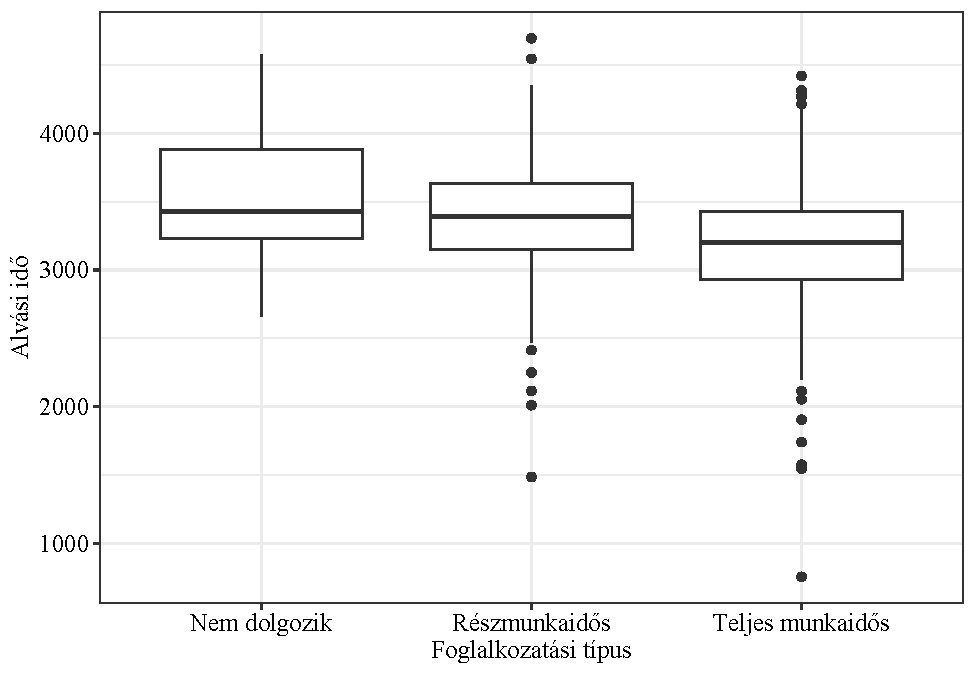
\includegraphics{econometrics_A2_files/figure-latex/unnamed-chunk-3-1.pdf}
\caption{Alvási idő dobozábrája foglalkozatatási típusonként}
\end{figure}

\hypertarget{b}{%
\subsection{b)}\label{b}}

\emph{Becsüljön meg három olyan regressziós modellt, amelyek függő
változója a sleep, és az első modell egyetlen magyarázó változója
totwrk, a második modell magyarázó változói totwrk és négyzete, a
harmadik modell pedig a foglalkoztatási kategóriákat tartalmazza
magyarázó változóként! (Természetesen minden modellben szerepeljen a
konstans is.) Megjegyzés: a factor() függvény hasznos lehet ebben a
részben.}

\begin{Shaded}
\begin{Highlighting}[]
\NormalTok{dat <-}\StringTok{ }\NormalTok{dat }\OperatorTok\StringTok{ }\KeywordTok{mutate}\NormalTok{(}\DataTypeTok{totwrk2 =}\NormalTok{ totwrk}\OperatorTok{^}\DecValTok{2}\NormalTok{)}
\NormalTok{model1 <-}\StringTok{ }\KeywordTok{lm}\NormalTok{(}\DataTypeTok{data =}\NormalTok{ dat, }\DataTypeTok{formula =}\NormalTok{ sleep }\OperatorTok{~}\StringTok{ }\NormalTok{totwrk)}
\NormalTok{model2 <-}\StringTok{ }\KeywordTok{lm}\NormalTok{(}\DataTypeTok{data =}\NormalTok{ dat, }\DataTypeTok{formula =}\NormalTok{ sleep }\OperatorTok{~}\StringTok{ }\NormalTok{totwrk }\OperatorTok{+}\StringTok{ }\NormalTok{totwrk2)}
\NormalTok{model3 <-}\StringTok{ }\KeywordTok{lm}\NormalTok{(}\DataTypeTok{data =}\NormalTok{ dat, }\DataTypeTok{formula =}\NormalTok{ sleep }\OperatorTok{~}\StringTok{ }\NormalTok{wrktype)}
\end{Highlighting}
\end{Shaded}

\hypertarget{c}{%
\subsection{c)}\label{c}}

\emph{Ábrázolja a sleep becsült függését a totwrk változótól egyetlen
ábrában a három modell alapján kiszámítva!}

\begin{Shaded}
\begin{Highlighting}[]
\KeywordTok{data.frame}\NormalTok{(}\DataTypeTok{sleep =}\NormalTok{ dat}\OperatorTok{$}\NormalTok{sleep, }\DataTypeTok{totwrk =}\NormalTok{ dat}\OperatorTok{$}\NormalTok{totwrk, }\DataTypeTok{m1 =}\NormalTok{ model1}\OperatorTok{$}\NormalTok{fitted.values,}
           \DataTypeTok{m2 =}\NormalTok{ model2}\OperatorTok{$}\NormalTok{fitted.values, }\DataTypeTok{m3 =}\NormalTok{ model3}\OperatorTok{$}\NormalTok{fitted.values) }\OperatorTok\StringTok{ }
\StringTok{  }\KeywordTok{pivot_longer}\NormalTok{(}\OperatorTok{-}\KeywordTok{c}\NormalTok{(}\DecValTok{1}\NormalTok{, }\DecValTok{2}\NormalTok{)) }\OperatorTok\StringTok{ }\KeywordTok{mutate}\NormalTok{(}
    \DataTypeTok{name =} \KeywordTok{paste0}\NormalTok{(}\KeywordTok{str_remove}\NormalTok{(name, }\StringTok{"m"}\NormalTok{), }\StringTok{". modell"}\NormalTok{) }
\NormalTok{  ) }\OperatorTok\StringTok{ }
\StringTok{  }\KeywordTok{ggplot}\NormalTok{(}\DataTypeTok{data =}\NormalTok{ .) }\OperatorTok{+}\StringTok{ }
\StringTok{  }\KeywordTok{geom_point}\NormalTok{(}\KeywordTok{aes}\NormalTok{(}\DataTypeTok{x =}\NormalTok{ totwrk, }\DataTypeTok{y =}\NormalTok{ sleep, }\DataTypeTok{fill =} \StringTok{"Valós értékek"}\NormalTok{),}
             \DataTypeTok{color =} \StringTok{'black'}\NormalTok{, }\DataTypeTok{shape =} \DecValTok{21}\NormalTok{) }\OperatorTok{+}
\StringTok{  }\KeywordTok{geom_line}\NormalTok{(}\KeywordTok{aes}\NormalTok{(totwrk, value, }\DataTypeTok{color =}\NormalTok{ name), }\DataTypeTok{size =} \DecValTok{2}\NormalTok{) }\OperatorTok{+}
\StringTok{  }\KeywordTok{scale_color_viridis_d}\NormalTok{() }\OperatorTok{+}
\StringTok{  }\KeywordTok{labs}\NormalTok{(}\DataTypeTok{x =} \StringTok{"Dolgozott munkaóra", y = "}\NormalTok{Alvási idő}\StringTok{", color = "}\NormalTok{Modellbecslés}\StringTok{", fill = "")}
\end{Highlighting}
\end{Shaded}

\begin{figure}
\centering
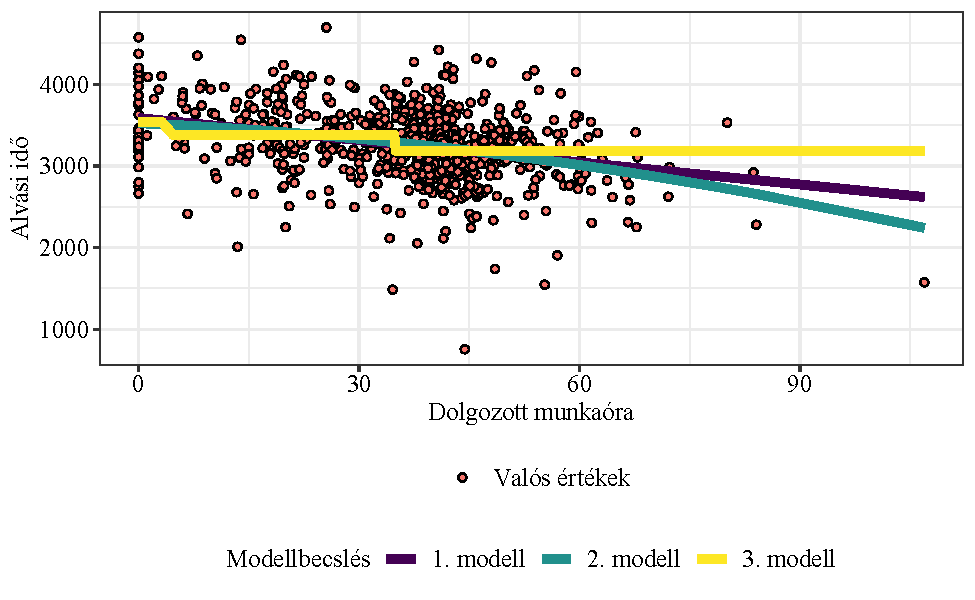
\includegraphics{econometrics_A2_files/figure-latex/unnamed-chunk-5-1.pdf}
\caption{Becsült alvási idő különböző modellekből}
\end{figure}

\hypertarget{d}{%
\subsection{d)}\label{d}}

\emph{Melyik modellt választaná a modellszelekciós kritériumok és az
értelmezhetőség alapján?}

\begin{Shaded}
\begin{Highlighting}[]
\KeywordTok{rbind}\NormalTok{(broom}\OperatorTok{::}\KeywordTok{glance}\NormalTok{(model1), broom}\OperatorTok{::}\KeywordTok{glance}\NormalTok{(model2)) }\OperatorTok
\StringTok{  }\KeywordTok{rbind}\NormalTok{(broom}\OperatorTok{::}\KeywordTok{glance}\NormalTok{(model3)) }\OperatorTok
\StringTok{  }\KeywordTok{mutate}\NormalTok{(}\DataTypeTok{model =} \KeywordTok{c}\NormalTok{(}\StringTok{"1. modell"}\NormalTok{, }\StringTok{"2. modell"}\NormalTok{, }\StringTok{"3. modell"}\NormalTok{)) }\OperatorTok
\StringTok{  }\KeywordTok{column_to_rownames}\NormalTok{(}\DataTypeTok{var =} \StringTok{'model'}\NormalTok{) }\OperatorTok
\StringTok{  }\KeywordTok{select}\NormalTok{(r.squared, adj.r.squared, AIC, BIC) }\OperatorTok
\StringTok{  }\KeywordTok{rename}\NormalTok{(}\KeywordTok{c}\NormalTok{(}\StringTok{"R négyzet"}\NormalTok{ =}\StringTok{ }\NormalTok{r.squared, }\StringTok{"Korrigált R négyzet"}\NormalTok{ =}\StringTok{ }\NormalTok{adj.r.squared)) }\OperatorTok\StringTok{ }
\StringTok{  }\NormalTok{knitr}\OperatorTok{::}\KeywordTok{kable}\NormalTok{(}\DataTypeTok{digits =} \DecValTok{4}\NormalTok{, }\DataTypeTok{format.args =} \KeywordTok{list}\NormalTok{(}\DataTypeTok{decimal.mark =} \StringTok{","}\NormalTok{),}
      \DataTypeTok{caption =}  \StringTok{"A 3 modell jellemzői"}\NormalTok{, }\DataTypeTok{align =} \KeywordTok{rep}\NormalTok{(}\StringTok{"c"}\NormalTok{, }\KeywordTok{ncol}\NormalTok{(.)))}
\end{Highlighting}
\end{Shaded}

\begin{longtable}[]{@{}lcccc@{}}
\caption{A 3 modell jellemzői}\tabularnewline
\toprule
& R négyzet & Korrigált R négyzet & AIC & BIC\tabularnewline
\midrule
\endfirsthead
\toprule
& R négyzet & Korrigált R négyzet & AIC & BIC\tabularnewline
\midrule
\endhead
1. modell & 0,1033 & 0,1020 & 10540,19 & 10553,87\tabularnewline
2. modell & 0,1075 & 0,1049 & 10538,90 & 10557,14\tabularnewline
3. modell & 0,0614 & 0,0588 & 10574,40 & 10592,64\tabularnewline
\bottomrule
\end{longtable}

A korrigált \(R^2\) az Akaike-féle információs mutató alapján alapján a
2. modellt, míg a BIC alapján az első modellt választanám. Mivel az
értelmezhetőség az első modell mellett szól (nincsen kvadratikus hatás,
így a \(\beta\)-kat egyszerűen lehet a parciális hatásként leolvasni),
így azt választanám.

\hypertarget{feladat-1}{%
\section{2. feladat}\label{feladat-1}}

\hypertarget{a-1}{%
\subsection{a)}\label{a-1}}

\emph{Becsüljön meg egy többváltozós regressziós modellt úgy, hogy az
alvással töltött idő a függő változó, és a munkával töltött idő, az
életkor, az életkor négyzete, az iskolázottság, a nem és a kisgyermek
jelenléte a magyarázó változó!}

\begin{Shaded}
\begin{Highlighting}[]
\NormalTok{model4 <-}\StringTok{ }\NormalTok{dat }\OperatorTok
\StringTok{  }\KeywordTok{mutate}\NormalTok{(}\DataTypeTok{age2 =}\NormalTok{ age}\OperatorTok{^}\DecValTok{2}\NormalTok{) }\OperatorTok\StringTok{ }
\StringTok{  }\NormalTok{\{dat <<-}\StringTok{ }\NormalTok{.\} }\OperatorTok\StringTok{ }\CommentTok{# refresh dat}
\StringTok{  }\KeywordTok{lm}\NormalTok{(}\DataTypeTok{formula =}\NormalTok{ sleep }\OperatorTok{~}\StringTok{ }\NormalTok{totwrk }\OperatorTok{+}\StringTok{ }\NormalTok{age }\OperatorTok{+}\StringTok{ }\NormalTok{age2 }\OperatorTok{+}\StringTok{ }\NormalTok{educ }\OperatorTok{+}\StringTok{ }\NormalTok{male }\OperatorTok{+}\StringTok{ }\NormalTok{yngkid)}
\end{Highlighting}
\end{Shaded}

\hypertarget{b-1}{%
\subsection{b)}\label{b-1}}

\emph{Értelmezze a nem és a kisgyermek jelenlétének paraméterbecslését!}

Ceteris paribus egy férfi várhatóan 8,7 perccel alszik többet, mint egy
nő. Amennyiben van kisgyermek, amely 3 évnél fiatalabb (yngkid = 1), úgy
az alvásidő várhatóan ceteris paribus 0,0228 perccel kevesebb.

\hypertarget{c-1}{%
\subsection{c)}\label{c-1}}

\emph{Tesztelje 5\%-os szinten, hogy a hibatag varianciája nem függ-e a
magyarázó változóktól!}

\begin{itemize}
\tightlist
\item
  \emph{Adja meg a tesztstatisztikát és a hozzá tartozó p-értéket!}
\item
  \emph{Értékelje a teszteredményt!}
\item
  \emph{Kell-e heteroszkedaszticitás-robusztus standard hibákat
  használni?}
\end{itemize}

\begin{Shaded}
\begin{Highlighting}[]
\NormalTok{lmtest}\OperatorTok{::}\KeywordTok{bgtest}\NormalTok{(model4)}
\end{Highlighting}
\end{Shaded}

A Breusch-Godfrey teszt-statisztikájának értéke (1) \textbf{0,6660},
amelyhez (1) \textbf{41,44\%-os} p-érték tartozik. Mivel jelen esetben a
(2) \textbf{nullhipotézist - mely szerint nincs heteroszkedaszticitás a
modellben - elfogadjuk minden gyakorlatban bevett
szignifikanciaszinten}, így a stanard hibákat tekinthetjük
torzítatlannak, és (3) \textbf{nem kell heteroszkedaszticitás-robusztus
standard hibákat használni}.

\hypertarget{d-1}{%
\subsection{d)}\label{d-1}}

\emph{Becsülje meg az alvással töltött időt egy 40 éves, teljes
munkaidőben dolgozó, kisgyerekes és középfokú végzettséggel (azaz 12
éves oktatással) rendelkező férfi munkavállaló számára!}

\begin{Shaded}
\begin{Highlighting}[]
\NormalTok{answer_2d <-}\StringTok{ }
\StringTok{  }\KeywordTok{data.frame}\NormalTok{(}\DataTypeTok{totwrk =} \DecValTok{35}\NormalTok{, }\DataTypeTok{age =} \DecValTok{40}\NormalTok{, }\DataTypeTok{age2 =} \DecValTok{40}\OperatorTok{^}\DecValTok{2}\NormalTok{, }\DataTypeTok{educ =} \DecValTok{12}\NormalTok{, }\DataTypeTok{male =} \DecValTok{1}\NormalTok{, }\DataTypeTok{yngkid =} \DecValTok{1}\NormalTok{) }\OperatorTok
\StringTok{  }\KeywordTok{predict.lm}\NormalTok{(}\DataTypeTok{object =}\NormalTok{ model4)}
\end{Highlighting}
\end{Shaded}

Egy 40 éves, teljes munkaidőben dolgozó, kisgyeremekes és középfokú
végzettséggel (azaz 12 éves oktatással) rendelkező férfi munkavállaló
várhatóan \textbf{3302,445} percet tölt hetente alvással.

\hypertarget{e}{%
\subsection{e)}\label{e}}

\emph{Adja meg a várható érték és a konkrét érték előrejelzésének
standard hibáját!}

\begin{Shaded}
\begin{Highlighting}[]
\KeywordTok{data.frame}\NormalTok{(}\DataTypeTok{totwrk =} \DecValTok{35}\NormalTok{, }\DataTypeTok{age =} \DecValTok{40}\NormalTok{, }\DataTypeTok{age2 =} \DecValTok{40}\OperatorTok{^}\DecValTok{2}\NormalTok{, }\DataTypeTok{educ =} \DecValTok{12}\NormalTok{, }\DataTypeTok{male =} \DecValTok{1}\NormalTok{, }\DataTypeTok{yngkid =} \DecValTok{1}\NormalTok{) }\OperatorTok
\StringTok{  }\KeywordTok{predict.lm}\NormalTok{(}\DataTypeTok{object =}\NormalTok{ model4, }\DataTypeTok{se.fit =}\NormalTok{ T, }\DataTypeTok{interval =} \StringTok{"confidence"}\NormalTok{) }\OperatorTok\StringTok{ }\NormalTok{.}\OperatorTok{$}\NormalTok{se.fit }\OperatorTok
\StringTok{  }\NormalTok{\{answer_3e_a <<-}\StringTok{ }\NormalTok{.\} }\OperatorTok\StringTok{ }
\StringTok{  }\NormalTok{\{answer_3e_b <<-}\StringTok{ }\NormalTok{. }\OperatorTok{+}\StringTok{ }\KeywordTok{sd}\NormalTok{(dat}\OperatorTok{$}\NormalTok{sleep)\}}
\end{Highlighting}
\end{Shaded}

A várható érték előrejelzésének standard hibája 52,69 perc, míg a
konkrét érték előrejelzésének standard hibája 497,1 perc.

\hypertarget{f}{%
\subsection{f)}\label{f}}

\emph{Adjon 95\%-os konfidencia-intervallumot a fenti két mennyiségre!}

\begin{Shaded}
\begin{Highlighting}[]
\KeywordTok{data.frame}\NormalTok{(}\DataTypeTok{totwrk =} \DecValTok{35}\NormalTok{, }\DataTypeTok{age =} \DecValTok{40}\NormalTok{, }\DataTypeTok{age2 =} \DecValTok{40}\OperatorTok{^}\DecValTok{2}\NormalTok{, }\DataTypeTok{educ =} \DecValTok{12}\NormalTok{, }\DataTypeTok{male =} \DecValTok{1}\NormalTok{, }\DataTypeTok{yngkid =} \DecValTok{1}\NormalTok{) }\OperatorTok
\NormalTok{\{}\KeywordTok{rbind}\NormalTok{(}\KeywordTok{predict.lm}\NormalTok{(}\DataTypeTok{object =}\NormalTok{ model4, }\DataTypeTok{newdata =}\NormalTok{ ., }\DataTypeTok{se.fit =}\NormalTok{ T, }\DataTypeTok{interval =} \StringTok{"confidence"}\NormalTok{)}\OperatorTok{$}\NormalTok{fit,}
\KeywordTok{predict.lm}\NormalTok{(}\DataTypeTok{object =}\NormalTok{ model4, }\DataTypeTok{newdata =}\NormalTok{ ., }\DataTypeTok{se.fit =}\NormalTok{ T, }\DataTypeTok{interval =} \StringTok{"prediction"}\NormalTok{)}\OperatorTok{$}\NormalTok{fit)\} }\OperatorTok\StringTok{ }
\StringTok{  }\KeywordTok{data.frame}\NormalTok{() }\OperatorTok\StringTok{ }
\StringTok{  }\KeywordTok{transmute}\NormalTok{(}\StringTok{"type"}\NormalTok{ =}\StringTok{ }\KeywordTok{c}\NormalTok{(}\StringTok{'Várható érték'}\NormalTok{, }\StringTok{'Konkrét érték'}\NormalTok{), lwr, upr) }\OperatorTok\StringTok{ }
\StringTok{  }\KeywordTok{mutate_at}\NormalTok{(}\OperatorTok{-}\DecValTok{1}\NormalTok{, }\ControlFlowTok{function}\NormalTok{(x) }\KeywordTok{format}\NormalTok{(x, }\DataTypeTok{decimal.mark =} \StringTok{','}\NormalTok{, }\DataTypeTok{digits =} \DecValTok{6}\NormalTok{)) }\OperatorTok\StringTok{ }
\StringTok{  }\KeywordTok{column_to_rownames}\NormalTok{(}\StringTok{'type'}\NormalTok{) }\OperatorTok\StringTok{ }
\StringTok{  }\KeywordTok{set_names}\NormalTok{(}\StringTok{'Alsó határ'}\NormalTok{, }\StringTok{'Felső határ'}\NormalTok{) }\OperatorTok\StringTok{ }
\StringTok{  }\NormalTok{knitr}\OperatorTok{::}\KeywordTok{kable}\NormalTok{(}\DataTypeTok{caption =} \StringTok{'Várható és konkrét érték konfidencia intervalluma'}\NormalTok{,}
               \DataTypeTok{align =} \KeywordTok{c}\NormalTok{(}\StringTok{'c'}\NormalTok{, }\StringTok{'c'}\NormalTok{))}
\end{Highlighting}
\end{Shaded}

\begin{longtable}[]{@{}lcc@{}}
\caption{Várható és konkrét érték konfidencia
intervalluma}\tabularnewline
\toprule
& Alsó határ & Felső határ\tabularnewline
\midrule
\endfirsthead
\toprule
& Alsó határ & Felső határ\tabularnewline
\midrule
\endhead
Várható érték & 3198,99 & 3405,90\tabularnewline
Konkrét érték & 2475,21 & 4129,68\tabularnewline
\bottomrule
\end{longtable}

\hypertarget{g}{%
\subsection{g)}\label{g}}

\emph{A (d) - (f) során melyik ponton feltételeztük a hibatag normális
eloszlását a számítások során?}

Az \textbf{f feladatban}.

\hypertarget{h}{%
\subsection{h)}\label{h}}

\emph{Vizsgálja meg egy megfelelő ábra segítségével, hogy a normalitás
feltételezése (hozzávetőlegesen) igaz-e!}

\begin{Shaded}
\begin{Highlighting}[]
\NormalTok{model4 }\OperatorTok
\StringTok{  }\NormalTok{broom}\OperatorTok{::}\KeywordTok{augment}\NormalTok{() }\OperatorTok\StringTok{ }\KeywordTok{select}\NormalTok{(.resid) }\OperatorTok\StringTok{ }
\StringTok{  }\NormalTok{\{}\KeywordTok{ggplot}\NormalTok{(}\DataTypeTok{data =}\NormalTok{ .)  }\OperatorTok{+}
\StringTok{  }\KeywordTok{stat_function}\NormalTok{(}\DataTypeTok{fun =}\NormalTok{ dnorm, }\DataTypeTok{args =} \KeywordTok{list}\NormalTok{(}\DataTypeTok{mean =} \KeywordTok{mean}\NormalTok{(.}\OperatorTok{$}\NormalTok{.resid), }\DataTypeTok{sd =} \KeywordTok{sd}\NormalTok{(.}\OperatorTok{$}\NormalTok{.resid)), }
  \KeywordTok{aes}\NormalTok{(}\DataTypeTok{fill =} \StringTok{'Hibatag átlagát és szórását követő normális eloszlás'}\NormalTok{),}
                    \DataTypeTok{geom =} \StringTok{'area'}\NormalTok{, }\DataTypeTok{alpha =} \FloatTok{.7}\NormalTok{, }\DataTypeTok{color =} \StringTok{"black"}\NormalTok{) }\OperatorTok{+}
\StringTok{    }\KeywordTok{geom_density}\NormalTok{(}\DataTypeTok{mapping =} \KeywordTok{aes}\NormalTok{(.resid, }\DataTypeTok{fill =} \StringTok{'Hibatag eloszlása'}\NormalTok{),}
                 \DataTypeTok{position =} \StringTok{'stack'}\NormalTok{, }\DataTypeTok{alpha =} \FloatTok{.4}\NormalTok{) }\OperatorTok{+}
\StringTok{    }\KeywordTok{scale_fill_viridis_d}\NormalTok{(}\DataTypeTok{direction =} \DecValTok{-1}\NormalTok{) }\OperatorTok{+}\StringTok{ }
\StringTok{    }\KeywordTok{labs}\NormalTok{(}\DataTypeTok{x =} \StringTok{""}\NormalTok{, }\DataTypeTok{y =} \StringTok{""}\NormalTok{, }\DataTypeTok{fill =} \StringTok{""}\NormalTok{)\}}
\end{Highlighting}
\end{Shaded}

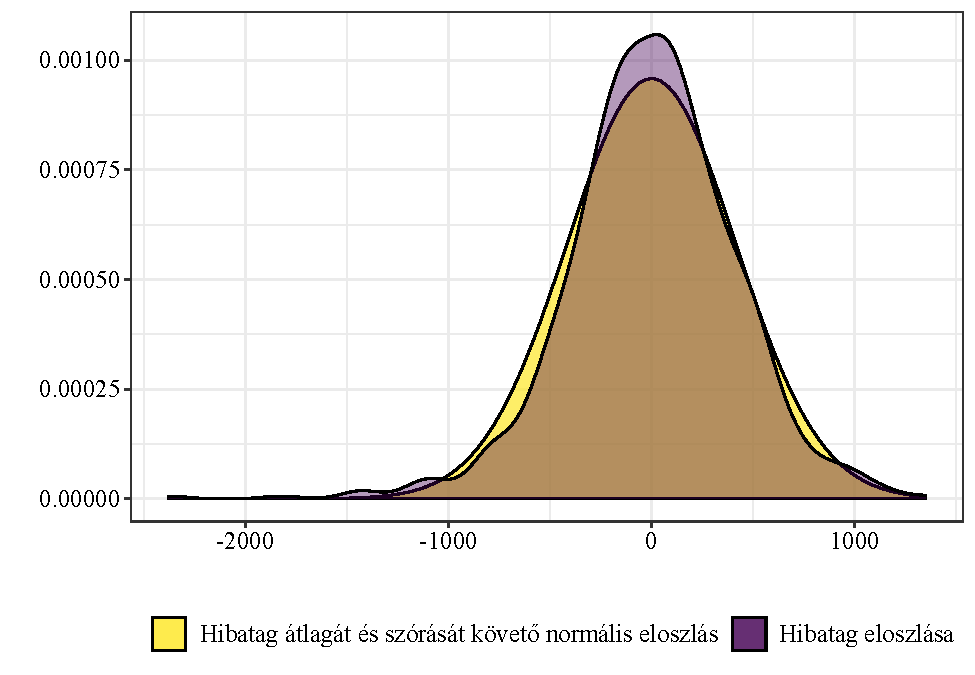
\includegraphics{econometrics_A2_files/figure-latex/unnamed-chunk-12-1.pdf}

\hypertarget{i}{%
\subsection{i)}\label{i}}

\emph{A mintát ossza fel véletlenszerűen két azonos méretű részre!
Becsülje meg a fenti modellt az egyik részmintán! Számítsa ki az átlagos
négyzetes eltérést (MSE) a becslési mintán és a másik (teszt-) mintán
is! Hasonlítsa össze az MSE értékeket és értelmezze az esetleges
különbséget!}

\begin{Shaded}
\begin{Highlighting}[]
\KeywordTok{set.seed}\NormalTok{(}\DecValTok{3}\NormalTok{)}
\NormalTok{dat }\OperatorTok
\StringTok{  }\KeywordTok{mutate}\NormalTok{(}\DataTypeTok{sample =} \KeywordTok{runif}\NormalTok{(}\DataTypeTok{n =} \KeywordTok{nrow}\NormalTok{(.)),}
  \DataTypeTok{sample =} \KeywordTok{ifelse}\NormalTok{(sample }\OperatorTok{<}\StringTok{ }\KeywordTok{median}\NormalTok{(sample), }\StringTok{'train'}\NormalTok{, }\StringTok{'test'}\NormalTok{)) }\OperatorTok\StringTok{ }
\StringTok{  }\NormalTok{\{dat <<-}\StringTok{ }\NormalTok{.\} }\OperatorTok\StringTok{ }
\StringTok{  }\KeywordTok{filter}\NormalTok{(sample }\OperatorTok{==}\StringTok{ 'train'}\NormalTok{) }\OperatorTok
\StringTok{  }\KeywordTok{lm}\NormalTok{(}\DataTypeTok{formula =}\NormalTok{ sleep }\OperatorTok{~}\StringTok{ }\NormalTok{totwrk }\OperatorTok{+}\StringTok{ }\NormalTok{age }\OperatorTok{+}\StringTok{ }\NormalTok{age2 }\OperatorTok{+}\StringTok{ }\NormalTok{educ }\OperatorTok{+}\StringTok{ }\NormalTok{male }\OperatorTok{+}\StringTok{ }\NormalTok{yngkid) }\OperatorTok
\StringTok{  }\NormalTok{\{model5 <<-}\StringTok{ }\NormalTok{.\}}

\KeywordTok{data.frame}\NormalTok{(}\StringTok{'Becslési minta'}\NormalTok{ =}\StringTok{ }\NormalTok{model5}\OperatorTok{$}\NormalTok{residuals,}
           \StringTok{'Teszt minta'}\NormalTok{ =}\StringTok{ }\KeywordTok{pull}\NormalTok{(}\KeywordTok{filter}\NormalTok{(dat, sample }\OperatorTok{==}\StringTok{ 'test'}\NormalTok{), sleep) }\OperatorTok{-}\StringTok{ }
\StringTok{            }\KeywordTok{predict.lm}\NormalTok{(}\DataTypeTok{object =}\NormalTok{ model5,}
            \DataTypeTok{newdata =} \KeywordTok{filter}\NormalTok{(dat, sample }\OperatorTok{==}\StringTok{ 'test'}\NormalTok{))) }\OperatorTok
\StringTok{  }\KeywordTok{apply}\NormalTok{(}\DecValTok{2}\NormalTok{, }\ControlFlowTok{function}\NormalTok{(x) }\KeywordTok{mean}\NormalTok{(x}\OperatorTok{^}\DecValTok{2}\NormalTok{)) }\OperatorTok\StringTok{ }\KeywordTok{matrix}\NormalTok{() }\OperatorTok\StringTok{ }\KeywordTok{t}\NormalTok{() }\OperatorTok\StringTok{  }
\StringTok{  }\KeywordTok{data.frame}\NormalTok{() }\OperatorTok\StringTok{ }\KeywordTok{set_names}\NormalTok{(}\KeywordTok{c}\NormalTok{(}\StringTok{'Becslési minta'}\NormalTok{, }\StringTok{'Teszt minta'}\NormalTok{)) }\OperatorTok\StringTok{ }
\StringTok{  }\KeywordTok{prtbl}\NormalTok{(}\StringTok{"MSE a becslési és a tesztmintán"}\NormalTok{, }\DataTypeTok{un =}\NormalTok{ F)}
\end{Highlighting}
\end{Shaded}

\begin{longtable}[]{@{}cc@{}}
\caption{MSE a becslési és a tesztmintán}\tabularnewline
\toprule
Becslési minta & Teszt minta\tabularnewline
\midrule
\endfirsthead
\toprule
Becslési minta & Teszt minta\tabularnewline
\midrule
\endhead
144697,7 & 208418,7\tabularnewline
\bottomrule
\end{longtable}

A teszt mintán számított MSE nagyobb, mint a becslési mintán, azonban ez
futtatásonként eltérő. Ennek oka a mintavételi ingadozás. Amennyiben ez
az eredmény gyakorta ismétlődik, úgy levonható következtetés lenne, hogy
a modell túlilleszkedik, de jelenleg nem levonható ez a következtetés,
mert ismételt mintavételek esetén előrfodul gyakran, hogy a teszt mintán
kisebb az MSE.

\hypertarget{feladat-2}{%
\section{3. feladat}\label{feladat-2}}

\hypertarget{a-2}{%
\subsection{a)}\label{a-2}}

\emph{Mennyivel különbözik a kisgyermekes és nem kisgyermekes szülők
alvással töltött átlagos ideje a férfiak illetve a nők esetében?}

\begin{Shaded}
\begin{Highlighting}[]
\NormalTok{dat }\OperatorTok\StringTok{ }\KeywordTok{group_by}\NormalTok{(male, yngkid) }\OperatorTok\StringTok{ }\KeywordTok{summarise}\NormalTok{(}\DataTypeTok{y =} \KeywordTok{mean}\NormalTok{(sleep)) }\OperatorTok
\StringTok{  }\KeywordTok{pivot_wider}\NormalTok{(}\DataTypeTok{names_from =} \StringTok{'yngkid'}\NormalTok{, }\DataTypeTok{values_from =} \StringTok{'y'}\NormalTok{) }\OperatorTok\StringTok{ }
\StringTok{  }\NormalTok{\{}\KeywordTok{data.frame}\NormalTok{(}\KeywordTok{c}\NormalTok{(}\StringTok{'nő'}\NormalTok{, }\StringTok{'férfi'}\NormalTok{),.[,}\DecValTok{2}\NormalTok{] }\OperatorTok{-}\StringTok{ }\NormalTok{.[,}\DecValTok{3}\NormalTok{])\} }\OperatorTok\StringTok{ }
\StringTok{  }\KeywordTok{set_names}\NormalTok{(}\StringTok{"Nem"}\NormalTok{, }\StringTok{"Különbség"}\NormalTok{) }\OperatorTok\StringTok{ }\KeywordTok{prtbl}\NormalTok{(}\StringTok{'Különbség a gyermek nemekre való hatásában'}\NormalTok{)}
\end{Highlighting}
\end{Shaded}

\begin{longtable}[]{@{}lc@{}}
\caption{Különbség a gyermek nemekre való hatásában}\tabularnewline
\toprule
Nem & Különbség\tabularnewline
\midrule
\endfirsthead
\toprule
Nem & Különbség\tabularnewline
\midrule
\endhead
nő & 66,74\tabularnewline
férfi & -12,09\tabularnewline
\bottomrule
\end{longtable}

\hypertarget{b-2}{%
\subsection{b)}\label{b-2}}

\emph{Egészítse ki a yngkid és a male interakciójával a 2. feladat
modelljét! Értelmezze a paraméterbecsléseket (és azok statisztikai
szignifikanciáját), majd hasonlítsa össze azokat a 2. feladat megfelelő
becslésével!}

\begin{Shaded}
\begin{Highlighting}[]
\KeywordTok{lm}\NormalTok{(}\DataTypeTok{data =}\NormalTok{ dat, }\DataTypeTok{formula =}\NormalTok{ sleep }\OperatorTok{~}\StringTok{ }\NormalTok{totwrk }\OperatorTok{+}\StringTok{ }\NormalTok{age }\OperatorTok{+}\StringTok{ }\NormalTok{age2 }\OperatorTok{+}\StringTok{ }\NormalTok{educ }\OperatorTok{+}\StringTok{ }\NormalTok{male }\OperatorTok{+}\StringTok{ }\NormalTok{yngkid }\OperatorTok{+}\StringTok{ }\NormalTok{yngkid}\OperatorTok{:}\NormalTok{male) }\OperatorTok\StringTok{ }
\StringTok{  }\NormalTok{broom}\OperatorTok{::}\KeywordTok{tidy}\NormalTok{() }\OperatorTok\StringTok{ }\KeywordTok{prtbl}\NormalTok{(}\StringTok{"A bővített modell paramétereinek becslése"}\NormalTok{)}
\end{Highlighting}
\end{Shaded}

\begin{longtable}[]{@{}lcccc@{}}
\caption{A bővített modell paramétereinek becslése}\tabularnewline
\toprule
Változó & Koefficiens & Standard hiba & T-statisztika &
P-érték\tabularnewline
\midrule
\endfirsthead
\toprule
Változó & Koefficiens & Standard hiba & T-statisztika &
P-érték\tabularnewline
\midrule
\endhead
konstans & 3861,00 & 239,85 & 16,10 & 0,00\%\tabularnewline
totwrk & -9,88 & 1,09 & -9,06 & 0,00\%\tabularnewline
age & -9,43 & 11,34 & -0,83 & 40,57\%\tabularnewline
age2 & 0,14 & 0,13 & 1,02 & 30,96\%\tabularnewline
educ & -11,38 & 5,88 & -1,94 & 5,31\%\tabularnewline
male & 74,56 & 36,22 & 2,06 & 3,99\%\tabularnewline
yngkid & -88,77 & 86,81 & -1,02 & 30,68\%\tabularnewline
male:yngkid & 128,04 & 102,12 & 1,25 & 21,03\%\tabularnewline
\bottomrule
\end{longtable}

Statisztikailag szignifikáns magyarázóváltozónka bizonyult a dolgozott
munkaóra és a nem 5\%-os szignifikanciaszinten. Az alvási időt csökkenti
a dolgozott heti munkaóra, ha az illető nő, ha van 3 évnél fiatalabb
gyermeke és az életkor növekedése kvadratikusan hat, kezdetben csökkenti
az alvási időt. A fő változás a 2 feladatban becsült modellhez képest,
hogy a fiatal gyermek jelenlétének paramétere jelentőset nőtt abszolút
értékben és a p-értéke is csökkent, bár a bevett szignifikanciaszinteken
még mindig nem szignifikáns. Ezzel szemben a férfi nem és fiatal gyermek
jelenlétének interakciójának paramétere pozitív előjelet kapott a
becsült modellben, amely arra utal, hogy a kisgyermek eltérő módon hat a
férfi és női szülő alvás idejére.

\hypertarget{feladat-3}{%
\section{4. feladat}\label{feladat-3}}

\emph{A titanic\_small.xls fájl tartalmazza a Titanic utasainak egyéni
jellemzőit: nem (sex=1 férfiak esetében, sex=2 nők esetében); az
osztály, amelyen utaztak (pclass), életkor (age) és hogy túléltéke a
katasztrófát (survived).}

\begin{Shaded}
\begin{Highlighting}[]
\NormalTok{dat <-}\StringTok{ }\NormalTok{rio}\OperatorTok{::}\KeywordTok{import}\NormalTok{(}\StringTok{'titanic_small.xls'}\NormalTok{)}
\end{Highlighting}
\end{Shaded}

\hypertarget{a-3}{%
\subsection{a)}\label{a-3}}

\emph{Számítsa ki a katasztrófát túlélő utazók százalékos arányát!
Mennyire különbözik ez osztályonként?}

\begin{Shaded}
\begin{Highlighting}[]
\NormalTok{dat }\OperatorTok\StringTok{ }\KeywordTok{group_by}\NormalTok{(pclass) }\OperatorTok\StringTok{ }\KeywordTok{summarise}\NormalTok{(}\DataTypeTok{r =} \KeywordTok{mean}\NormalTok{(survived)) }\OperatorTok\StringTok{ }\KeywordTok{mutate}\NormalTok{(}
  \DataTypeTok{r =}\NormalTok{ scales}\OperatorTok{::}\KeywordTok{percent}\NormalTok{(r, }\DataTypeTok{decimal.mark =} \StringTok{','}\NormalTok{, }\DataTypeTok{accuracy =} \FloatTok{.01}\NormalTok{)) }\OperatorTok\StringTok{ }
\StringTok{  }\KeywordTok{set_names}\NormalTok{(}\StringTok{"Osztály"}\NormalTok{, }\StringTok{"Túlélési arány"}\NormalTok{) }\OperatorTok\StringTok{ }\KeywordTok{prtbl}\NormalTok{(}\StringTok{"Túlélési arány utazási osztályonként"}\NormalTok{)}
\end{Highlighting}
\end{Shaded}

\begin{longtable}[]{@{}cc@{}}
\caption{Túlélési arány utazási osztályonként}\tabularnewline
\toprule
Osztály & Túlélési Arány\tabularnewline
\midrule
\endfirsthead
\toprule
Osztály & Túlélési Arány\tabularnewline
\midrule
\endhead
1 & 61,92\%\tabularnewline
2 & 42,96\%\tabularnewline
3 & 25,53\%\tabularnewline
\bottomrule
\end{longtable}

\hypertarget{b-3}{%
\subsection{b)}\label{b-3}}

\emph{Becsüljön meg egy lineáris valószínűségi modellt (LPM), egy logit
és egy probit modellt, függő változóként a túlélés valószínűségét,
magyarázó változóként pedig az osztályt (mint kategorikus változót), a
nemet és az életkort használva!}

\begin{Shaded}
\begin{Highlighting}[]
\NormalTok{lpm <-}\StringTok{ }\NormalTok{dat }\OperatorTok\StringTok{ }\KeywordTok{lm}\NormalTok{(}\DataTypeTok{formula =}\NormalTok{ survived}\OperatorTok{~}\KeywordTok{factor}\NormalTok{(pclass)}\OperatorTok{+}\KeywordTok{factor}\NormalTok{(sex)}\OperatorTok{+}\NormalTok{age)}
\NormalTok{logit <-}\StringTok{ }\NormalTok{dat }\OperatorTok\StringTok{ }\KeywordTok{glm}\NormalTok{(}\DataTypeTok{formula =}\NormalTok{ survived}\OperatorTok{~}\KeywordTok{factor}\NormalTok{(pclass)}\OperatorTok{+}\KeywordTok{factor}\NormalTok{(sex)}\OperatorTok{+}\NormalTok{age,}
            \DataTypeTok{family =} \KeywordTok{binomial}\NormalTok{(}\DataTypeTok{link =} \StringTok{"logit"}\NormalTok{))}
\NormalTok{probit <-}\StringTok{ }\NormalTok{dat }\OperatorTok\StringTok{ }\KeywordTok{glm}\NormalTok{(}\DataTypeTok{formula =}\NormalTok{ survived}\OperatorTok{~}\KeywordTok{factor}\NormalTok{(pclass)}\OperatorTok{+}\KeywordTok{factor}\NormalTok{(sex)}\OperatorTok{+}\NormalTok{age,}
            \DataTypeTok{family =} \KeywordTok{binomial}\NormalTok{(}\DataTypeTok{link =} \StringTok{"probit"}\NormalTok{))}
\end{Highlighting}
\end{Shaded}

\hypertarget{c-2}{%
\subsection{c)}\label{c-2}}

\emph{Számítsa ki az LPM, logit és probit modellek alapján a
harmadosztályon és a másodosztályon utazók átlagos kontrollált
túlélésvalószínűség-különbségét!}

\begin{Shaded}
\begin{Highlighting}[]
\KeywordTok{merge}\NormalTok{(lpm }\OperatorTok\StringTok{ }\NormalTok{broom}\OperatorTok{::}\KeywordTok{tidy}\NormalTok{() }\OperatorTok
\StringTok{  }\KeywordTok{transmute}\NormalTok{(term, }\DataTypeTok{LPM =}\NormalTok{ estimate),}
\NormalTok{mfx}\OperatorTok{::}\KeywordTok{logitmfx}\NormalTok{(}\DataTypeTok{atmean =}\NormalTok{ F, }\DataTypeTok{data =}\NormalTok{ dat,}
  \DataTypeTok{formula =}\NormalTok{ survived }\OperatorTok{~}\StringTok{ }\KeywordTok{factor}\NormalTok{(pclass) }\OperatorTok{+}\StringTok{ }\KeywordTok{factor}\NormalTok{(sex) }\OperatorTok{+}\StringTok{ }\NormalTok{age) }\OperatorTok\StringTok{ }
\StringTok{  }\NormalTok{.}\OperatorTok{$}\NormalTok{mfxest }\OperatorTok\StringTok{ }\KeywordTok{data.frame}\NormalTok{() }\OperatorTok\StringTok{ }\KeywordTok{rownames_to_column}\NormalTok{() }\OperatorTok\StringTok{ }
\StringTok{  }\KeywordTok{select}\NormalTok{(}\DecValTok{1}\OperatorTok{:}\DecValTok{2}\NormalTok{) }\OperatorTok\StringTok{ }\KeywordTok{set_names}\NormalTok{(}\StringTok{'term'}\NormalTok{, }\StringTok{'Logit'}\NormalTok{)}
\NormalTok{) }\OperatorTok\StringTok{ }\KeywordTok{merge}\NormalTok{(}
\NormalTok{  mfx}\OperatorTok{::}\KeywordTok{probitmfx}\NormalTok{(}\DataTypeTok{atmean =}\NormalTok{ F, }\DataTypeTok{data =}\NormalTok{ dat,}
  \DataTypeTok{formula =}\NormalTok{ survived }\OperatorTok{~}\StringTok{ }\KeywordTok{factor}\NormalTok{(pclass) }\OperatorTok{+}\StringTok{ }\KeywordTok{factor}\NormalTok{(sex) }\OperatorTok{+}\StringTok{ }\NormalTok{age) }\OperatorTok\StringTok{ }
\StringTok{  }\NormalTok{.}\OperatorTok{$}\NormalTok{mfxest }\OperatorTok\StringTok{ }\KeywordTok{data.frame}\NormalTok{() }\OperatorTok\StringTok{ }\KeywordTok{rownames_to_column}\NormalTok{() }\OperatorTok\StringTok{ }
\StringTok{  }\KeywordTok{select}\NormalTok{(}\DecValTok{1}\OperatorTok{:}\DecValTok{2}\NormalTok{) }\OperatorTok\StringTok{ }\KeywordTok{set_names}\NormalTok{(}\StringTok{'term'}\NormalTok{, }\StringTok{'Probit'}\NormalTok{)}
\NormalTok{) }\OperatorTok\StringTok{ }\KeywordTok{filter}\NormalTok{(}
\NormalTok{  term }\OperatorTok{==}\StringTok{ 'factor(pclass)2'} \OperatorTok{|}\StringTok{ }\NormalTok{term }\OperatorTok{==}\StringTok{ 'factor(pclass)3'}
\NormalTok{) }\OperatorTok\StringTok{ }\KeywordTok{mutate}\NormalTok{(}\DataTypeTok{term =} \KeywordTok{str_remove}\NormalTok{(term, }\StringTok{'factor}\CharTok{\textbackslash{}\textbackslash{}}\StringTok{(pclass}\CharTok{\textbackslash{}\textbackslash{}}\StringTok{)'}\NormalTok{)) }\OperatorTok\StringTok{ }
\StringTok{  }\KeywordTok{mutate_at}\NormalTok{(}\OperatorTok{-}\DecValTok{1}\NormalTok{, }\ControlFlowTok{function}\NormalTok{(x) scales}\OperatorTok{::}\KeywordTok{percent}\NormalTok{(x, }\DataTypeTok{accuracy =} \FloatTok{.01}\NormalTok{, }\DataTypeTok{decimal.mark =} \StringTok{','}\NormalTok{)) }\OperatorTok\StringTok{ }
\StringTok{  }\KeywordTok{rename}\NormalTok{(}\StringTok{'Osztály'}\NormalTok{ =}\StringTok{ }\NormalTok{term) }\OperatorTok\StringTok{ }
\StringTok{  }\KeywordTok{prtbl}\NormalTok{(}\DataTypeTok{align =} \KeywordTok{c}\NormalTok{(}\StringTok{'c'}\NormalTok{, }\StringTok{'c'}\NormalTok{, }\StringTok{'c'}\NormalTok{, }\StringTok{'c'}\NormalTok{))}
\end{Highlighting}
\end{Shaded}

\begin{longtable}[]{@{}cccc@{}}
\toprule
Osztály & Lpm & Logit & Probit\tabularnewline
\midrule
\endhead
2 & -21,14\% & -18,14\% & -18,64\%\tabularnewline
3 & -37,04\% & -36,68\% & -35,97\%\tabularnewline
\bottomrule
\end{longtable}

\hypertarget{d-2}{%
\subsection{d)}\label{d-2}}

\emph{Hasonlítsa össze ezt a három számot egymással és az a) rész
eredményeivel!}

A 3 modell alapján készült kontrolállt valószínűség-különbség jól
közelíti a sokkaságban megfigyelhető arányokat. Az eltérés fő oka a
magyarázóváltozók közötti multikollinearitás, de itt ez most nem
számottevő.

\hypertarget{e-1}{%
\subsection{e)}\label{e-1}}

\emph{A klasszifikációhoz használja a 0,5 értéket küszöbként. Számítsa
ki a logit modell alapján a kétfajta klasszifikációs hibát és a helyesen
besorolt megfigyelések arányát!}

\begin{Shaded}
\begin{Highlighting}[]
\NormalTok{regclass}\OperatorTok{::}\KeywordTok{confusion_matrix}\NormalTok{(}\DataTypeTok{M =}\NormalTok{ logit, }\DataTypeTok{DATA =}\NormalTok{ dat) }\OperatorTok
\StringTok{  }\NormalTok{\{.[}\OperatorTok{-}\DecValTok{3}\NormalTok{,}\OperatorTok{-}\DecValTok{3}\NormalTok{]\} }\OperatorTok
\StringTok{  }\NormalTok{\{(.}\OperatorTok{/}\KeywordTok{sum}\NormalTok{(.))\} }\OperatorTok\StringTok{ }
\StringTok{  }\KeywordTok{data.frame}\NormalTok{(}\DataTypeTok{row.names =} \KeywordTok{c}\NormalTok{(}\StringTok{'Valós 0'}\NormalTok{, }\StringTok{'Valós 1'}\NormalTok{)) }\OperatorTok\StringTok{ }
\StringTok{  }\KeywordTok{rownames_to_column}\NormalTok{() }\OperatorTok\StringTok{ }
\StringTok{  }\KeywordTok{mutate_at}\NormalTok{(}\OperatorTok{-}\DecValTok{1}\NormalTok{, }\ControlFlowTok{function}\NormalTok{(x) scales}\OperatorTok{::}\KeywordTok{percent}\NormalTok{(x, }\DataTypeTok{accuracy =} \FloatTok{.01}\NormalTok{, }\DataTypeTok{decimal.mark =} \StringTok{','}\NormalTok{)) }\OperatorTok\StringTok{ }
\StringTok{  }\KeywordTok{column_to_rownames}\NormalTok{() }\OperatorTok\StringTok{ }
\StringTok{  }\KeywordTok{set_names}\NormalTok{(}\KeywordTok{c}\NormalTok{(}\StringTok{'Becsült 0'}\NormalTok{, }\StringTok{'Becsült 1'}\NormalTok{)) }\OperatorTok\StringTok{ }
\StringTok{  }\NormalTok{knitr}\OperatorTok{::}\KeywordTok{kable}\NormalTok{(}\DataTypeTok{caption =} \StringTok{'A logit modellel készített kalsszifikáció konfúziós mátrixa'}\NormalTok{, }\DataTypeTok{align =} \KeywordTok{c}\NormalTok{(}\StringTok{'c'}\NormalTok{, }\StringTok{'c'}\NormalTok{))}
\end{Highlighting}
\end{Shaded}

\begin{longtable}[]{@{}lcc@{}}
\caption{A logit modellel készített kalsszifikáció konfúziós
mátrixa}\tabularnewline
\toprule
& Becsült 0 & Becsült 1\tabularnewline
\midrule
\endfirsthead
\toprule
& Becsült 0 & Becsült 1\tabularnewline
\midrule
\endhead
Valós 0 & 49,71\% & 9,46\%\tabularnewline
Valós 1 & 12,05\% & 28,78\%\tabularnewline
\bottomrule
\end{longtable}

A táblázatból kiolvasható, hogy a helyesen besoroltak aránya 78\%, a
hibásan klasszifikált valóságban 1-esek aránya 12\%, míg a hibásan
klasszifikált 0-sok aránya 10\%.

\end{document}
